\section{Method} 
\label{sec:method}
In this section, we introduce our logic-aware RAG system, named HopRAG. An overview of this system is illustrated in Figure \ref{fig:overview}.
\begin{figure*}[htbp!]
\centering
  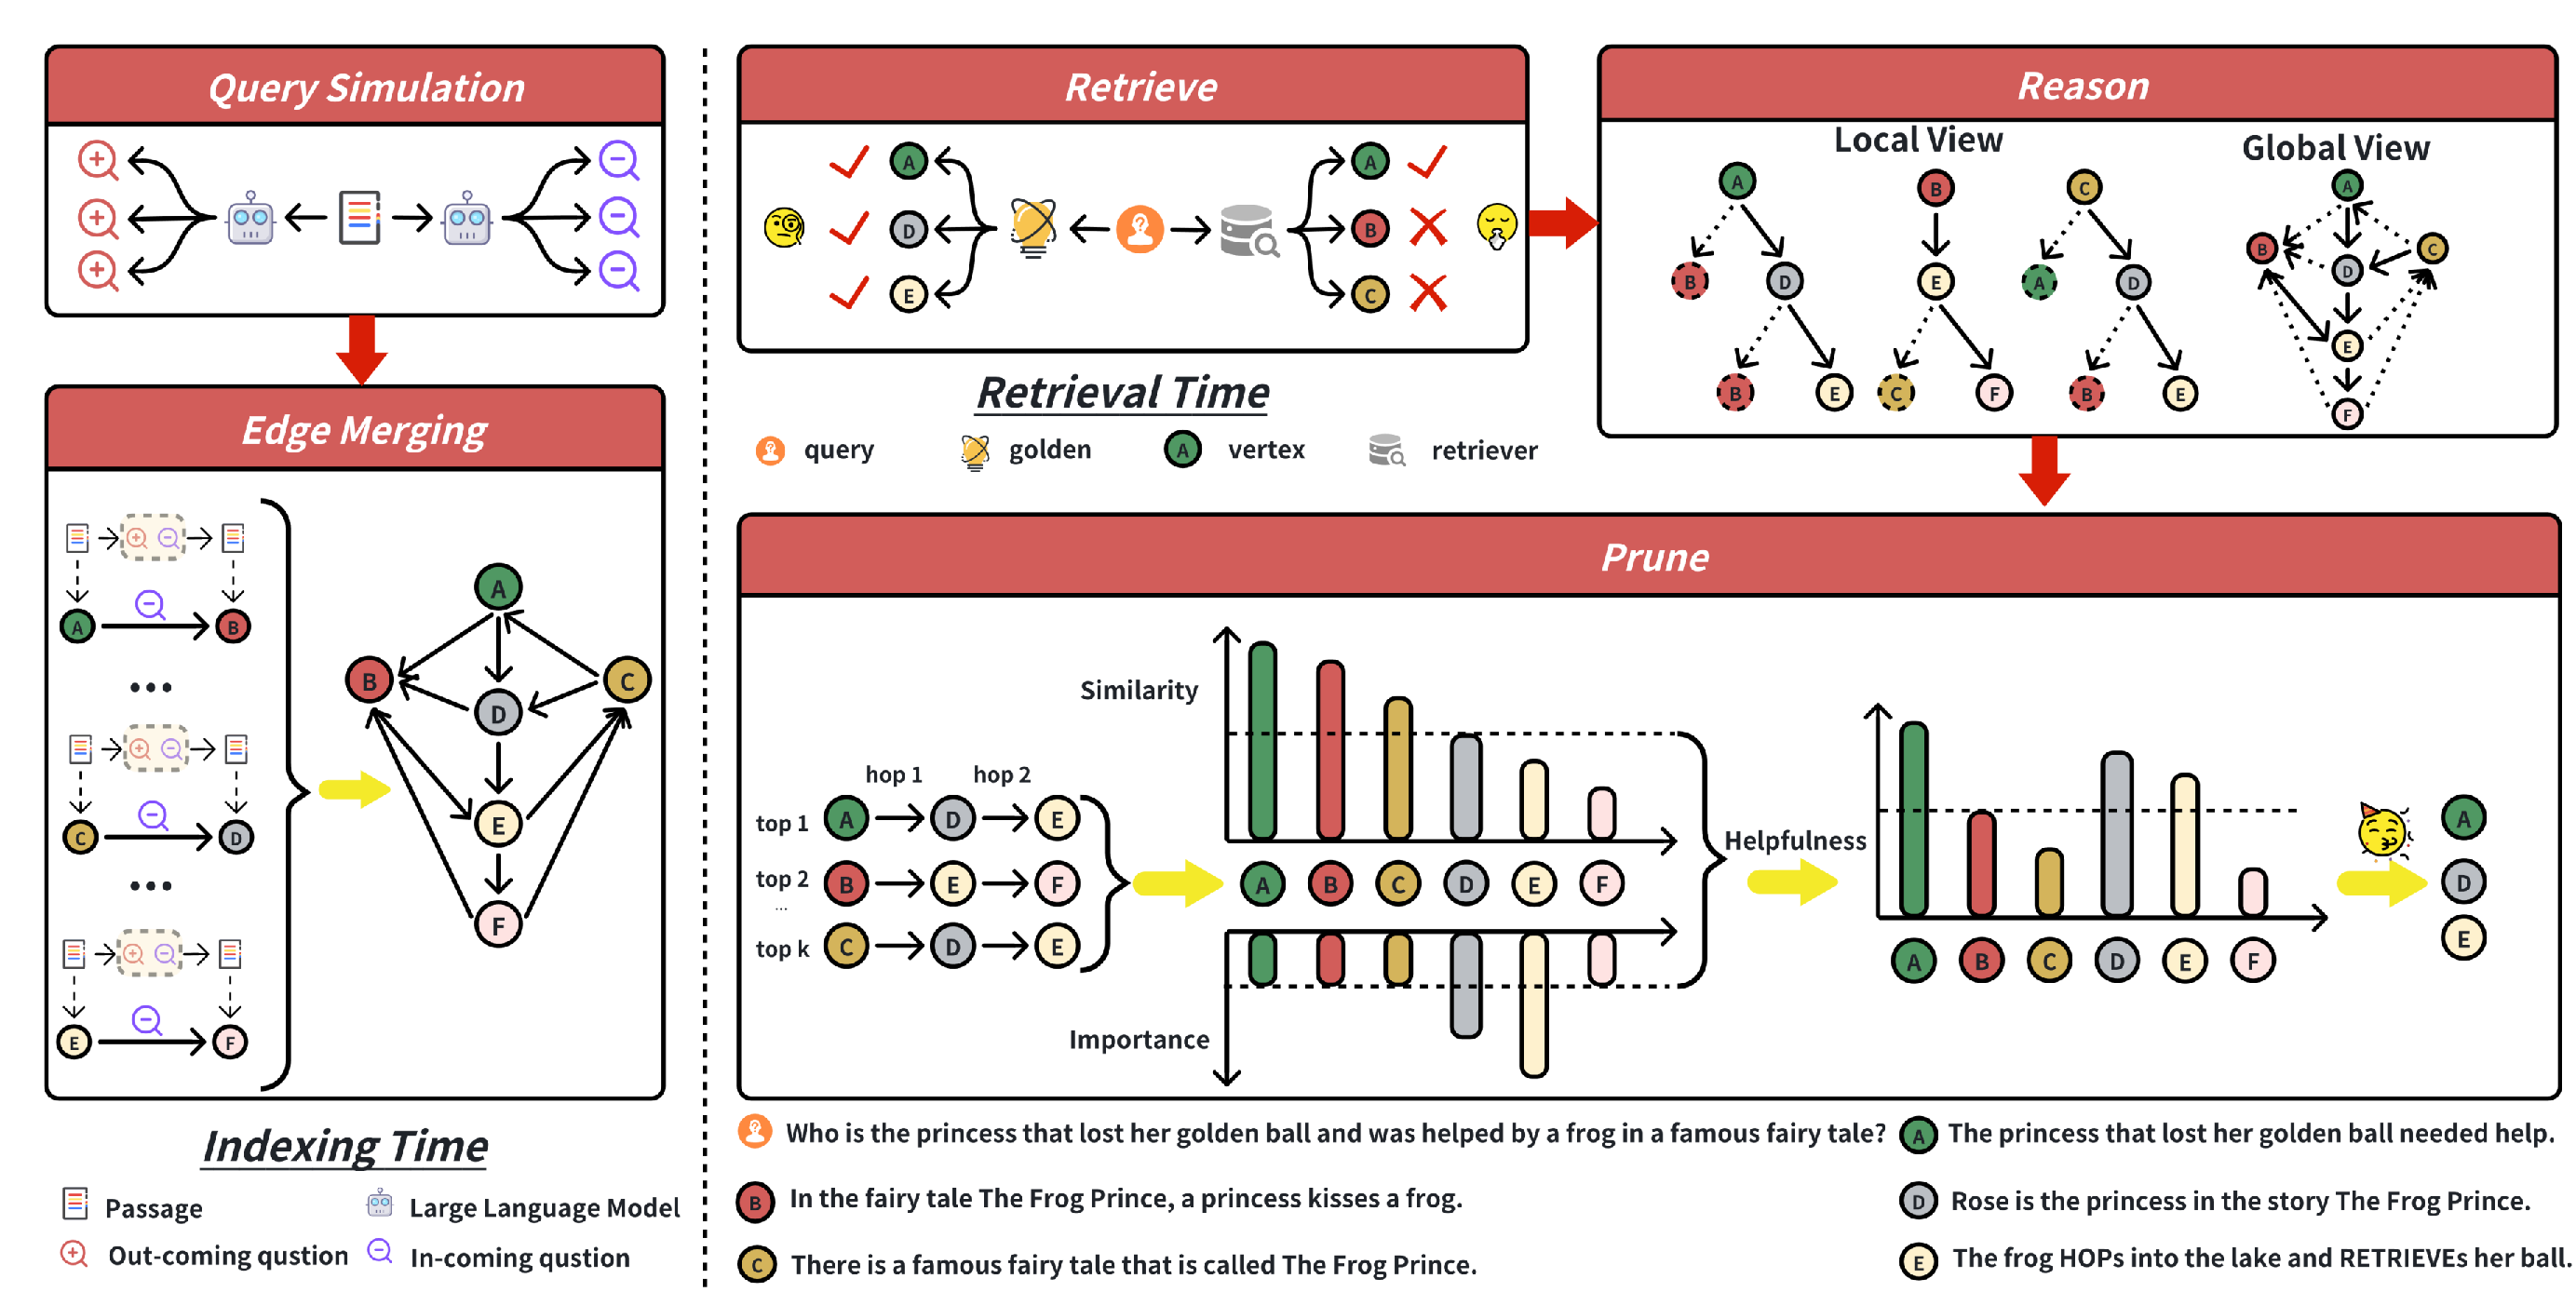
\includegraphics[width=\textwidth]{latex/figures/overview_nm.pdf}
  \caption{The workflow of HopRAG. \textbf{Left:} At indexing time, we first utilize \textit{Query Simulation} to generate pseudo-queries for each passage and then apply \textit{Edge Merging} to connect passages with directed logical edges. \textbf{Right:} At retrieval time, we employ a \textit{Retrieve-Reason-Prune} pipeline. We first retrieve through purely similarity-based retrieval, then run reasoning-augmented graph traversal to explore the neighborhood, and finally prune the search by a novel metric \textit{Helpfulness} considering both textual similarity and logical importance.}
  \label{fig:overview}
\end{figure*}
\subsection{Problem Formulation}

Given a passage corpus $P=\{p_1, p_2, ..., p_N\}$ and a query $q$ which requires the information from multiple passages in $P$, the task is to design (1) a graph-structured RAG knowledge base that not only stores all the passages in corpus $P$ but also models the similarity and logic between passages; (2) a corresponding retrieval strategy that can hop from indirectly relevant passages to truly relevant passages for better retrieval. Finally, with the query $q$ and $k$ passages as context ${C}=\{p_{i_1},p_{i_2},...,p_{i_k}\}$, the LLM generates the response \(\mathcal{O} \sim \mathcal{P}(\mathcal{O}|q, {C}) \).

\subsection{Graph-Structured Index}
We construct a graph-structured index $G=(\mathcal{V},\mathcal{E})$ where the vertex set $\mathcal{V}$ consists of vertices storing all the passages and the directed edge set $\mathcal{E} = \{\langle v_i,e_{i,j},v_j\rangle | v_i,v_j\in \mathcal{V} \}\subset \mathcal{V} \times \mathcal{V}$ is established based on the logical relations between passages for multi-hop reasoning. To establish $G$, we utilize \textbf{Query Simulation} to identify the logical relations and leverage textual similarity for efficient \textbf{Edge Merging}. 
\paragraph{Query Simulation}
To identify the logical relations between passages, we generate a series of pseudo-queries for each passage, and use them to explore the passage's relations with the others and bridge the inherent gap between user-queries and passages \citep{wang_qaencoder_2024}. Specifically, we adopt LLM to generate two groups of pseudo-queries for each passage $p_i$: (1) $m$ out-coming questions $Q_i^+= \bigcup_{1 \le j \le m} \{q_{i,j}^{+} \}$ that originate from this passage but cannot be answered by itself; (2) $n$ in-coming questions $Q_i^-= \bigcup_{1 \le j \le n} \{q_{i,j}^{-}\}$ whose answers are within the passage. As demonstrated in Figure \ref{fig:demo}, for the toy passage "Rose is the princess in the story The Frog Prince", one in-coming question might be "What is the name of the princess?" and one out-coming question might be "How is the frog connected to Rose?". The prompts are in Appendix \ref{prompt}. 

We extract keywords from $Q_i^+$ and $Q_i^-$ using named entity recognition $\text{NER}(\cdot)$ for sparse representation, and embed these questions into semantic vectors using an embedding model $\text{EMB}(\cdot)$ for dense representation. This results in sparse representations $K_i^+= \bigcup_{1 \le j \le m}\{k_{i,j}^{+} \}$ and $K_i^-= \bigcup_{1 \le j \le n}\{k_{i,j}^{-}\}$, and dense representations $V_i^+=\bigcup_{1 \le j \le m} \{\mathbf{v}_{i,j}^{+}\}$ and $V_i^-=\bigcup_{1 \le j \le n} \{\mathbf{v}_{i,j}^{-}\}$. We further define out-coming triplets as $r_{i,j}^+:=(q_{i,j}^{+},k_{i,j}^{+},\mathbf{v}_{i,j}^{+})$ and in-coming triplets $r_{i,j}^-:=(q_{i,j}^{-},k_{i,j}^{-},\mathbf{v}_{i,j}^{-})$. Each passage $p_i$ is stored inside a vertex $v_i$, featured with its out-coming triplets $R_i^+= \bigcup_{1 \le j \le m} \{r_{i,j}^{+}\}$ and in-coming triplets $R_i^-= \bigcup_{1 \le j \le n} \{r_{i,j}^{-} \}$. 

\paragraph{Edge Merging}
Given the out-coming and in-coming triplets, we match paired triplets via hybrid retrieval and establish directed edges between the corresponding passages.
For each out-coming triplet $r_{s,i}^+$ of source vertex $v_s$, the most matching in-coming triplet $r_{t^*,j^*}^-$ is determined as follows:
\begin{equation}
\label{sim}
\begin{aligned}
    \text{SIM}(r_{s,i}^{+}, r_{t,j}^{-}) &= \frac{\frac{|k_{s,i}^{+} \cap k_{t,j}^{-}|}{|k_{s,i}^{+} \cup k_{t,j}^{-}|}+\frac{\mathbf{v}_{s,i}^{+} \cdot \mathbf{v}_{t,j}^{-}}{||\mathbf{v}_{s,i}^{+}|| \cdot ||\mathbf{v}_{t,j}^{-}||}}{2} \\
    r_{t^*,j^*}^- &= \arg\max_{r_{t,j}^{-}  } \text{SIM}(r_{s,i}^{+}, r_{t,j}^{-})
\end{aligned}
\end{equation}

We then build the directed edge $\langle v_s,e_{s,t^*},v_{t^*} \rangle$ with aggregated features, where $e_{s,t^*}:=({q_{t^*,j^*}^{-}},{k_{t^*,j^*}^{-}\cup k_{s,i}^{+}},{\mathbf{v}_{t^*,j^*}^{-}})$. 

\subsection{Reasoning-Augmented Graph Traversal }
For more accurate and complete responses, HopRAG's retrieval strategy leverages the reasoning ability of LLM to explore the neighborhood of probably indirectly relevant passages and hop to relevant ones based on the logical relations in the graph structure. As shown in Algorithm \ref{ragt}, by reasoning over the questions on out edges $e_{i,j}$ of a current vertex $v_{i}$ and then choosing to hop to the most promising vertex $v_{j}$, we realize reasoning-augmented graph traversal for better retrieval performance. 

\paragraph{Retrieval Phase} To start the local search over the graph for query $q$, we first use $\text{NER}(\cdot)$ and $\text{EMB}(\cdot)$ to get the keywords $ k_{q}$ and vector $\mathbf{v}_{q}$ of $q$, which will be used for hybrid retrieval to match $top_k$ similar edges $\langle v_i,e_{i,j},v_j \rangle $, following Equation \ref{sim}. With each vertex $v_j$ from these edges we initialize a context queue $C_{queue}$ for breadth-first local search \citep{voudouris2010guided}. 

\paragraph{Reasoning Phase} To fully exploit the logical relations over the graph and hop from indirectly relevant vertices to relevant ones, we introduce breadth-first local search which utilizes the LLM to choose the most appropriate neighbor for each $v_j$ in $C_{queue}$ to append to the tail of the queue. Specifically, for each $v_j$ in $C_{queue}$ in each round of hop, we leverage LLM to reason over all the questions from its out edges to choose one $e_{j,k}$ with the question which the LLM regards as the most helpful for answering $q$ and append vertex $v_k$ to $C_{queue}$.  
After hopping from each vertex in the current $C_{queue}$ we can expand the context with at most $top_k$ new vertices. From these new vertices we continue the next round of hop. Since different vertices may hop to the same vertex, we believe the vertices with more visits are more important for answering $q$, and use a counter $C_{count}$ to track the number of visits for each vertex and measure its importance. By conducting $n_{hop}$ rounds of hop, we realize reasoning-augmented graph traversal and expand the context length to at most $(n_{hop}+1)\times top_k$.

\paragraph{Pruning Phase} To avoid including too many intermediate vertices during the traversal, we introduce a novel metric Helpfulness $H(\cdot)$  that integrates similarity and logic to re-rank and then prune the traversal counter $C_{count}$. We calculate $H_i$ following Equation \ref{H} for each $v_i$ in $C_{count}$ and keep the $top_k$ vertices with the highest $H_i$, where hybrid textual similarity $\text{SIM}(v_i, q)$ calculates the average lexical and semantic similarity between the passage in $v
_i$ and query $q$ following Equation \ref{sim}; and $\text{IMP}(v_i,C_{count})$ is defined as the normalized number of visits of $v_i$ in $C_{count}$ during traversal following Equation \ref{Imp}. We prune \( C_{count} \) by retaining $top_k$ vertices with the highest \( H \) value, resulting in the final context \( C \).

\begin{equation}
    H_i=\frac{\text{SIM}(v_i, q)+\text{IMP}(v_i,C_{count})}{2}
    \label{H}
\end{equation}
\begin{equation}
    \text{IMP}(v_i, C_{count}) = \frac{C_{count}[v_i]}{\sum_{v_j \in C_{count}} C_{count}[v_j]}
    \label{Imp}
\end{equation}
\begin{algorithm}
  \SetAlgoLined
  \KwIn{$q$, $top_k$, $n_{hop}$, $G$}
  \KwOut{$C$}
 $\mathbf{v}_{q}$ $\leftarrow$ EMB($q$)\;$  k_{q}$ $\leftarrow$ NER($q$)\;
  $C_{queue}\leftarrow$ Retrieve($\mathbf{v}_{q}$, $k_{q}$, $G$)\;
  $C_{count}\leftarrow $Counter$(C_{queue})$\;
  \For{$i \leftarrow 1,2,...,n_{hop}$ }{
  \For{j $\leftarrow 1,2,...,\mid C_{queue}\mid $} {
  $v_j\leftarrow $ $C_{queue}$.dequeue()\;
  $v_k \leftarrow$ Reason($\{\langle v_j,e_{j,k},v_k\rangle\}$)\;
\eIf{$v_k$  not in $C_{count}$}{
$C_{queue}$.enqueue($v_k$)\;
$C_{count}[v_k]\leftarrow1$ \;
      }{
      $C_{count}[v_k]++$ \;
      }
  }
  }
  $C\leftarrow$Prune($C_{count}$, $\mathbf{v}_{q}$, $k_q$, $top_k$)\;
  \Return $C$
  \caption{Reasoning-Augmented Graph Traversal}
  \label{ragt}
\end{algorithm}
